   \section{Simulation} 
We performed a Monte Carlo study to investigate the performance our proposed estimator and compare it with its alternatives. 

Consider a data set $D = \{(x_i, y_i), i = 1,..., N\}$, consisting of a predictor $x_i\in\mathcal{L}_2$ and a scalar response $y_i$ that follow the model: 
 \begin{equation} \label{eq:gen}
y_i = r(x_i) + \rho \epsilon_i,
\end{equation}
where errors $\epsilon_i$ are i.i.d distributed and  $\rho > 0$ is a constant that controls the signal-to-noise ratio (SNR): 
$$\text{SNR} = \frac{\text{Var}(r(X))}{\text{Var}(\rho\epsilon)}.$$
We fixed SNR = 5 and considered $x_i$ generated form the model 

 $$x_i(t) = \mu(t) + \sum_{p=1}^4 \sqrt{\lambda_j}\xi_{ij}\phi_j(t),$$
where $\mu(t) = 2\text{sin}(t\pi) \text{exp}(1-t)$, $\lambda_1 = 0.8, \lambda_2 = 0.3, \lambda_3 = 0.2$, and $\lambda_4 = 0.1$,  $\xi_{ij}\sim N(0,1) $,  and $\phi_j$ are the first four eigenfunctions of the ``Mattern'' covariance function $\gamma(s,t)$ with parameters $\rho = 3, \sigma = 1, \nu = 1/3$: 
 $$\gamma(s,t) = C\left(\frac{\sqrt{2\nu}|s-t|}{\rho}\right), \ C(u) = \frac{\sigma^2 2^{1-\nu}}{\Gamma(\nu)} u^{\nu} K_{\nu}(u),$$
  where $\Gamma(.)$ is the Gamma distribution and $K_{\nu}$ is the modified Bessel function of the second kind.
  
 We considered four regression functions to generate the response: 
\mathleft
\begin{equation*}
\hspace{15ex}
	r_1(X) =  \int_{\mathcal{I}} \left (\text{sin} \left(\frac{3}{2} \pi t \right) +  \text{sin} \left(\frac{1}{2} \pi t \right)\right)X(t)dt,
\end{equation*}
\mathleft
\begin{equation*}
\hspace{15ex}
	r_2(X) = 5\text{exp}\left (- \frac{1}{2}\left| \int_{\mathcal{I}} x(t)\log(|x(t)|)dt \right| \right),
\end{equation*}
\mathleft
\begin{equation*}
\hspace{15ex}
r_3(X) = (\xi_1 + \xi_2)^{1/3},
\end{equation*}
where  $\xi_1 = \int_{\mathcal{I}} (X(t) - \mu(t))\psi_1(t) dt$ and $\xi_2 = \int_{\mathcal{I}} (X(t) - \mu(t))\psi_2(t) dt$ are projections to the first two FPCs ($\psi_1$ and $\psi_2$,) of $X$ with mean  $\mu(t) = E(X(t))$, 
\begin{equation*}
\hspace{15ex}
r_4(X) = 5 \left( \sqrt{\left|\int_{\mathcal{I}_1} \text{cos}(2\pi t^2) X(t) dt \right|} + \sqrt{\left|\int_{\mathcal{I}_2} \text{sin}(X(t)) dt \right|} \right),
\end{equation*}
where  $\mathcal{I}_1 = [0,0.5]$ and $\mathcal{I}_2 = (0.5,1]$. 


We considered the following error distributions: 

\begin{itemize}
 \setlength\itemsep{0em}
\item $D_0$: Clean - $\epsilon \sim N(0,1)$
\item $D1$: Symmetric gross errors - $\epsilon \sim 0.8 N(0,1) + 0.1 N(20,0.1^2) + 0.1 N(-20, 0.1^2)$ 
\item $D_2$: Asymmetric gross errors - $\epsilon \sim 0.8 N(0,1) + 0.2 N(20,0.1^2)$ 
\end{itemize}
and compared four estimators 
\begin{itemize}
\itemsep0em 
\item \texttt{TFBoost(L2)}: tree-based functional boosting with L2 loss
\item \texttt{TFBoost(LAD)}: tree-based functional boosting with LAD loss
\item \texttt{TFBoost(RR)}: robust tree-based functional boosting (MM-type)
\item \texttt{RobustFPLM}: robust semi-functional linear estimator proposed by \cite{boente2020robust}
\end{itemize}
We initialize \texttt{TFBoost(RR)} with type B functional multi-index tree that minimizes the average absolute value of the residuals. We refer to it as \texttt{LADTree}.  We considered \texttt{LADTrees} with depth 0, 1, 2, 3 and 4, and the minimum number of observations per node set at 10, 20 or 30 (note that an LADTree of depth 0 corresponds to using the median of the responses as the initial fit). Of the 13 different combinations we chose the one that performs the best on the validation set. As the validation set may also contain outliers, we first fitted a depth 0 tree and trimmed as potential outliers those observations with residuals deviating from their median by more than 3 times their MAD.


For each of the 12 possible combinations of the regression function and error distribution, we constructed training, validation, and test sets of size 400, 200, and 1000 respectively.   Test sets were always generated with uncontaminated data $D_0$. Each estimator was fitted using the training and validation sets, while the test sets were reserved to evaluate the performance of the different estimators.   

The results for all methods under consideration are given in terms of the MSPE on the test set ($\mathcal{T}$): $\text{MSPE}_{\text{test}} = \frac{1}{|\mathcal{T}|} \sum_{i \in \mathcal{T}} (\hat{F}(x_i) - y_i)^2$.  In particular, for \texttt{TFBoost}, the estimate $\hat{F}$ is evaluated at the early stopping time, which was determined by the loss evaluated on the validation set.  

MSPE on the test sets in different settings are plotted below (y axis is truncated):

\begin{figure}[H]
\centering
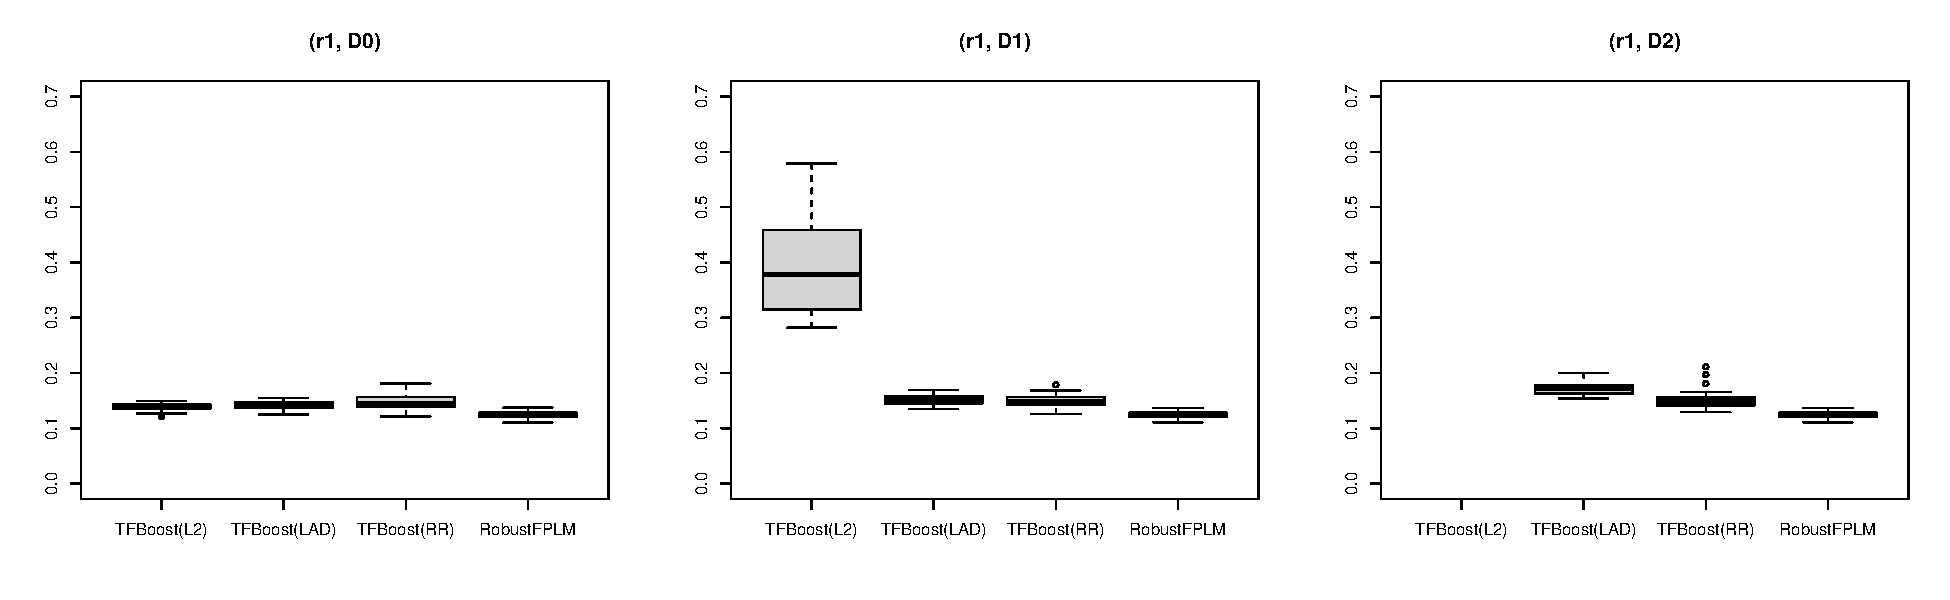
\includegraphics[scale = 0.56, page = 1]{figs/sim.pdf}
\caption{test MSPE for $r_1$ with no contamination ($D_0$), symmetric contamination ($D_1$), and asymmetric contamination ($D_2$)}
\end{figure}


\begin{figure}[H]
\centering
\includegraphics[scale = 0.56, page = 2]{figs/sim.pdf}
\caption{test MSPE for $r_2$  with no contamination ($D_0$), symmetric contamination ($D_1$), and asymmetric contamination ($D_2$)}
\end{figure}


\begin{figure}[H]
\centering
\includegraphics[scale = 0.56, page = 3 ]{figs/sim.pdf}
\caption{test MSPE for $r_3$  with no contamination ($D_0$), symmetric contamination ($D_1$), and asymmetric contamination ($D_2$)}
\end{figure}


\begin{figure}[H]
\centering
\includegraphics[scale = 0.56, page = 4]{figs/sim.pdf}
\caption{test MSPE for $r_4$  with no contamination ($D_0$), symmetric contamination ($D_1$), and asymmetric contamination ($D_2$)}
\end{figure}





 